\documentclass[12pt]{article}
\usepackage{fontspec}
\usepackage{polyglossia}
\usepackage{geometry}
\usepackage{xcolor}
\usepackage{titlesec}
\usepackage{fancyhdr}
\usepackage{graphicx}
\usepackage{mathtools}
\graphicspath{{../matlab/figures/}}
\usepackage{hyperref} % Add hyperref package for clickable links
\usepackage{amsmath}
\usepackage{tabularx}

\usepackage{float}
\usepackage{caption}
\usepackage{subcaption}

% Set the page margins
\geometry{margin=2.54cm}

%\usepackage{kmath,kerkis} % The order of the packages matters; kmath changes the default text font
%\usepackage[T1]{fontenc}

% Set the font to Kerkis
\setmainfont{Calibri}


\usepackage{matlab-prettifier}
\newfontfamily\greekfonttt[Script=Greek]{Calibri}

% Define colors
\definecolor{myblue}{RGB}{0, 51, 102}
\definecolor{mygray}{RGB}{150,150,150}
\definecolor{mybg}{RGB}{230,230,230}

% Set section title formatting
\titleformat{\section}
  {\normalfont\Large\bfseries\color{myblue}}
  {\thesection}{1em}{}
%\titleformat{\subsection}
%  {\normalfont\Large\bfseries\color{myblue}}
%  {\thesubsection}{1em}{}

\setmainlanguage{greek}
\setotherlanguage{english}

% Define header and footer
\pagestyle{fancy}
\fancyhf{}
\lhead{Ομάδα 2}
\rhead{Υλοποίηση εξελικτικού πρωταθλήματος Axelrod}
\rfoot{\thepage}

%\title{Αναφορά εργαστηρίου}
%\author{Όνομα Φοιτητή}
%\date{\today}

\begin{document}
\begin{titlepage}
\newgeometry{margin=2cm, tmargin=3cm, bmargin=3cm}
\centering
\begin{figure}[H]
\centering

\includegraphics[width=0.8\textwidth]{banner-horizontal-black300ppi.png}\par % Image on top of title
\end{figure}
%\textcolor{black}{\large \bfseries Αριστοτέλειο Πανεπιστήμιο Θεσσαλονίκης\\}\par
\vspace{18pt}
\textcolor{black}{\Large \bfseries Τμήμα Ηλεκτρολόγων Μηχανικών\\και Μηχανικών Υπολογιστών\\}\par
\vspace{1cm}
\vfill
\textcolor{black}{\Large \bfseries Θεωρία Παιγνίων}\par
\vspace{12pt}
\textcolor{black}{\large \bfseries Υλοποίηση εξελικτικού πρωταθλήματος Axelrod}\par

\vspace{0.5cm} % Adjust vertical spacing here
\vfill
\newcolumntype{L}{>{\raggedright\arraybackslash}X}%
\newcolumntype{R}{>{\raggedleft\arraybackslash}X}%
{\large
\def\arraystretch{1.3}
\begin{tabularx}{\textwidth}{ R|L }
\textbf{Ομάδα}                			 & 2           \\
\textbf{Βαπόρης Δημήτριος}      & ΑΕΜ 10625 \\
\textbf{Βουλκίδης Βλάσιος}        & ΑΕΜ 10627 \\
\textbf{Ντελόπουλος Εμμανουήλ}      & ΑΕΜ 10693 \\
\textbf{Υπεύθυνος Καθηγητής}           & Κεχαγιάς Αθανάσιος\\
\end{tabularx}
}
\vspace{0.5cm}
\vfill
\textcolor{black}{\large \bfseries Εαρινό Εξάμηνο 2025}\par
\end{titlepage}
\restoregeometry

\tableofcontents % Table of Contents

\newpage
\section{Εισαγωγή}
Το συγκεκριμένο αρχείο είναι η αναφορά της εργασίας για το μάθημα Θεωρία Παιγνίων. Αντικείμενο της εργασίας αυτής είναι η υλοποίηση και η μελέτη του εξελικτικού πρωταθλήματος Axelrod στο παίγνιο "Δίλημμα του Φυλακισμένου". Με την ονομασία αυτή χαρακτηρίζεται το κοινωνικό δίλημμα, δηλαδή οποιοδήποτε παίγνιο της μορφής $\begin{bmatrix} A_{1,1} & A_{1,2} \\ A_{2,1} & A_{2,2} \end{bmatrix}$, τιμές για τις οποίες ισχύει $ A_{1,2} < A_{2,2} < A_{1,1} < A_{2,1}$. Η επανάληψη του παιγνίου αυτού δημιουργεί ένα match μεταξύ στρατηγικών, matches μεταξύ στρατηγικών δημιουργούν τουρνουά μεταξύ στρατηγικών και ο υπολογισμός νέου πληθυσμού με βάση την επίδοση κάθε στρατηγικής στο τουρνουά αποτελεί το αντικείμενο μελέτης της εργασίας. 

Η εργασία αποτελείται από 4 βασικές συναρτήσεις, κάθε μία από τις οποίες επιτελεί μία συγκεκριμένη λειτουργία που μπορεί να χαρακτηριστεί από δύο χαρακτηριστικά της εκάστοτε παραδοχής: η φύση της προσομοίωσης (θεωρητική ή πραγματική) και η εξελικτική δυναμική (fitness ή imitation). Συγκεκριμένη εισαγωγή γίνεται και κατά την παρουσίαση της κάθε συνάρτησης, στην οποία εξηγείται ο τρόπος λειτουργίας και τυχούσες παραδοχές που συνέβησαν σε κάθε περίπτωση. Το πρώτο μέρος της εργασίας βασίζεται σε σημαντικό ποσοστό στη μελέτη των Mathieu et al. Μάλιστα, καταβλήθηκε προσπάθεια τα αποτελέσματα να είναι κατά το δυνατόν όμοια με αυτά που παρουσιάζει το paper του 1999.

\section{Fitness Dynamics}

Πρώτη εξελικτική δυναμική που θα αναλυθεί (και αυτή που αναλύεται από τους Mathieu et al.) είναι η δυναμική του fitness, σύμφωνα με την οποία ανατίθεται σε κάθε στρατηγική της προσομοίωσης ένα score, το οποίο χρησιμοποιείται ώστε να υπολογστεί η κατανομή του πληθυσμού της επόμενης γενιάς. Ακολουθείται και για τις δύο παρακάτω συναρτήσεις που αξιοποιούν το fitness η θεώρηση των Mathieu et al, σύμφωνα με την οποία το fitness κάθε στρατηγικής υπολογίζεται ως εξής: 

Έστω ότι ο πληθυσμός απαρτίζεται από 3 στρατηγικές, την A, την B και την C. Υπολογίζονται με βάση τον πίνακα του παιγνίου B, τον αριθμό των γύρων κάθε αγώνα T και, προφανώς, των στρατηγικών που βρίσκονται "αντιμέτωπες" σε κάθε περίπτωση, οι απολαβές κάθε μίας από τις 2 στρατηγικές και αποθηκεύονται ως π.χ. V(A|B), η απολαβή της στρατηγικής A όταν συναντά την B. Έπειτα, το score κάθε παίκτη που χρησιμοποιεί την εκάστοτε στρατηγική (και άρα, ουσιαστικά, της στρατηγικής) υπολογίζεται ως, π.χ. για τη στρατηγική A, $g_n(A) = W_n(A)V(A|A) + W_n(B)V(A|B) + W_n(C)V(A|C) − V(A|A)$ , όπου $W_n(A), W_n(B), W_n(C)$ οι πληθυσμοί της εκάστοτε στρατηγικής στη γενιά $n$ (παρατηρήστε ότι αφαιρείται μία φορά η απολαβή για παιχνίδι με την ίδια στρατηγική του κάθε παίκτη, διότι θεωρείται ότι παραλείπεται το παιχνίδι με τον εαυτό του κάθε μέλους του πληθυσμού). Τέλος, το συνολικό score του τουρνουά υπολογίζεται ως $t(n) = W_n(A)g_n(A) + W_n(B)g_n(B) + W_n(C)g_n(C)$ και ο πληθυσμός της γενιάς $n+1$ για π.χ. τη στρατηγική A γίνεται $W_{n+1}(A) = \frac{\Pi W_n(A)g_n(A)}{t(n)}$. 

Να επισημανθεί εδώ ότι η λογική αυτή εφαρμόζεται λόγω της πλήρους ντετερμινιστικής φύσης των στρατηγικών που έχουν υλοποιηθεί: εάν υπήρχαν στρατηγικές με τυχαίο στοιχείο, ο θεωρητικός υπολογισμός των αποτελεσμάτων κάθε αγώνα θα ήταν αδύνατος και θα έπρεπε να υπολογιστεί κάποια αναμενόμενη τιμή, αντικείμενο που ξεφεύγει από το αντικείμενο μελέτης της εργασίας.
\subsection{Η συνάρτηση TourSimFit}
Πρώτη συνάρτηση που υλοποιείται είναι η [POP,BST,FIT]=TourSimFit(B,Strategies,POP0,T,J), όπου B ο πίνακας απολαβών του παιγνίου, Strategies ένα array από Strings με τα ονόματα των στρατηγικών που συμμετέχουν στην προσομοίωση, POP0 ο αρχικός πληθυσμός, T ο αριθμός γύρων σε κάθε αγώνα και J ο αριθμός γενεών του εξελικτικού πρωταθλήματος. Επιστρέφονται τα εξής: POP ένας πίνακας με τους πληθυσμούς κάθε στρατηγικής ανά γενεά, BST πίνακας που περιλαμβάνει τις καλύτερες στρατηγικές κάθε γύρου (0 αν δεν ανήκει στις καλύτερες, 1 αν ανήκει στις καλύτερες, οι ισοπαλίες μετράνε) και FIT ένας πίνακας με τα fitness scores κάθε στρατηγικής για κάθε γενεά. Η λογική της συνάρτησης ακολουθεί όσα παρουσιάστηκαν παραπάνω, όμως προστίθεται κατά τον υπολογισμό των πληθυσμών της επόμενης γενιάς λογική ώστε να αποφεύγεται η ύπαρξη δεκαδικών και ο πληθυσμός κάθε στρατηγικής σε κάθε γενιά να παραμένει ακέραιος. Η λογική λειτουργεί ως εξής:

Λαμβάνεται ως αρχικό αποτέλεσμα των παραπάνω πράξεων για τον πληθυσμό το floor των δεκαδικών αποτελεσμάτων. Έπειτα, υπολογίζεται τυχόν έλλειμμα που προκύπτει από την εφαρμογή της συνάρτησης floor και ανατίθεται ένας ανά φορά νέος παίκτης σε κάποια στρατηγική τυχαία, μέχρις ότου να μηδενιστεί το έλλειμμα. Γίνεται και έλεγχος για το αν η στρατηγική βρίσκεται ήδη σε μηδενικό πληθυσμό, ώστε να αποφευχθεί η "αναγέννησή" της. Έτσι, ο συνολικός πληθυσμός των παικτών παραμένει σταθερός καθ' όλη τη διάρκεια της προσομοίωσης, όπως θεωρούν και οι Mathieu et al.

Η επιλογή αυτή γίνεται συνειδητά. Δοκιμάστηκαν οι περιπτώσεις κατά τις οποίες ανατίθεται κάθε παίκτης στη στρατηγική η οποία έχει πληθυσμό πιο κοντά στον επόμενο ακέραιο (π.χ. αν κάποια στρατηγική είχε αρχικά υπολογσιμένο πληθυσμό 199.8, αυτό να μετατραπεί σε 200), όπως και η ακριβώς αντίθετη περίπτωση, όπου δηλαδή ανατίθεται στη στρατηγική πιο μακριά από τον επόμενο ακέραιο. Οι αλγόριθμοι αυτοί παρουσίασαν μερικές ανεπιθύμητες συμπεριφορές διατήρησης ενός πολύ χαμηλού αριθμού παικτών συγκεκριμένων στρατηγικών (π.χ. κάποια στρατηγική να κολλάει σε πληθυσμό 2 επειδή ο αρχικά υπολογισμένος πληθυσμός επόμενης γενεάς είναι 1.8, ή αντίστοιχα π.χ. 1.1). Διατηρώντας αυτό το τυχαίο στοιχείο, τα αποτελέσματα των προσομοιώσεων δεν παρουσιάζουν σημαντική διαφορά με αυτά δίχως τυχαιότητα, ενώ παράλληλα η μέθοδος εγγυάται ότι σε βάθος χρόνου οι "αδύναμες" στρατηγικές εξαφανίζονται πλήρως.

Παρατηρώντας, ωστόσο, την απόκλιση της υλοποίησης αυτής από τα αποτελέσματα του paper, προσθέσαμε την εξής μετατροπή: ένα έξτρα όρισμα τύπου boolean στη συνάρτηση TourSimFit, με την ονομασία compensation και default τιμή false, το οποίο επιτελεί τη λειτουργία που περιγράφεται παρακάτω. Με τιμή false, επιστρέφει τα αποτελέσματα μόνο με απλό rounding στον κοντινότερο μικρότερο ακέραιο (rounding προς τα κάτω), το οποίο θεωρούμε ότι γίνεται και στο paper. Στην περίπτωση αυτή, ο πληθυσμός ανά γενιά δεν παραμένει υποχρεωτικά σταθερός, αλλά η απόκλιση δεν αυξάνεται με προσθετικό τρόπο. Ίσως χάνονται απλά 1 ή 2 μέλη του πληθυσμού σε μερικές γενιές, λόγω του round down. Με τιμή true,  επιστρέφει τα αποτελέσματα σύμφωνα με τη λογική ανάθεσης των χαμένων μελών που περιγράφηκε παραπάνω. Στις προσομοιώσεις που ακολουθούν, παρουσιάζεται και μία σύγκριση των 2 αυτών μεθόδων με τα αποτελέσματα της συνάρτησης TourTheFit, που περιγράφεται παρακάτω. Θεωρήθηκε περιττή η προσθήκη των αποτελεσμάτων του paper.

\subsection{Η συνάρτηση TourTheFit}
Η δεύτερη συνάρτηση που υλοποιήθηκε είναι η [POP,BST,FIT]=TourTheFit(B,Strategies,POP0,T,J), με ορίσματα και εξόδους παντελώς πανομοιότυπα με αυτά της προηγούμενης. Η μόνη ουσιαστική διαφορά κείτεται στο ότι πλέον, λόγω της θεωρητικής φύσης της προσομοίωσης, παραλείπεται το τμήμα του κώδικα που ήταν υπεύθυνο για τη διατήρηση ακεραίων στον πληθυσμό, καθώς επιτρέπονται και οι δεκαδικοί αριθμοί, αφού ο πληθυσμός δεν αποτελείται πραγματικά από παίκτες.

\subsection{Προσομοίωσεις}
Παρακάτω ακολουθούν οι προσομοιώσεις για την περίπτωση των fitness dynamics, οι οποίες ακολουθούν κατά πολύ τη λογική των Mathieu et al. Στόχος ήταν να επιτευχθεί όσο το δυνατόν πιστή αντιγραφή των αποτελεσμάτων που παρουσιάζονται στο paper. Για τον σκοπό αυτό, ως default τιμή του πίνακα απολαβών χρησιμοποιήθηκε $B = \begin{bmatrix} 3 & 0 \\5 & 1 \end{bmatrix}$ και προστέθηκαν στη λίστα των 12 στρατηγικών που είχαν έως τώρα υλοποιηθεί οι στρατηγικές per\_ccd, per\_ddc, soft\_majo και per\_ccccd, οι οποίες χρησιμοποιούνται δεόντως στο paper. Η κάθε προσομοίωση βρίσκεται στο αρχείο example.m σε κατάλληλο Section και με Run Section προκύπτουν ακριβώς τα αποτελέσματα που παρουσιάζονται παρακάτω.
\subsubsection{1η Προσομοίωση - Defectors may be strong}
Ήδη από την πρώτη προσομοίωση, παρουσιάζεται ένα ενδιαφέρον αποτέλεσμα. Σκοπός της προσομοίωσης αυτής είναι να αναδείξει ότι σε συγκεκριμένα σύνολα στρατηγικών και βολικές αρχικές τιμές πληθυσμού, λιποτακτικές στρατηγικές όπως η per\_ddc είναι ικανές να κυριαρχήσουν. Ωστόσο, η θεωρητική ανάλυση της περίπτωσης που μελετάται στο paper δε δείχνει ακριβώς αυτήν την εικόνα. Αυτό οφείλεται στο γεγονός ότι ο πληθυσμός soft\_majo στις περιπτώσεις των προσομοιώσεων εξαφανίζεται εντελώς περίπου στην 20η γενιά, ενώ στη θεωρητική περίπτωση αυτό δε συμβαίνει. Έτσι, μετά από κάποια γενιά και μία σχετική μείωση του πληθυσμού per\_ddc, επιστρέφει η στρατηγική soft\_majo και αναπτύσσεται η στρατηγική Alternator, που ουσιαστικά είναι και ο τέλειος αντίπαλος της soft\_majo, διότι διαπράττει ακριβώς όσες λιποταξίες μπορεί για να διατηρήσει τη soft\_majo σε συνεργασία. Μετά από ένα σημείο, βέβαια, αρχίζουν και πάλι οι 2 πληθυσμοί αυτοί να μειώνονται και να αυξάνεται ο πληθυσμός των per\_ddc, κάτι που μας κάνει να υποψιαζόμαστε ότι το παράδειγμα αυτό θεωρητικά οδηγείται σε ταλάντωση. Στις προσομοιώσεις, όμως, και στην περίπτωση του compensation και στην άλλη, τα αποτελέσματα είναι πολύ παρόμοια με αυτά του paper: η ελαφριά διαφοροποίηση στην περίπτωση του compensation οφείλεται στο τυχαίο στοιχείο, το οποίο κάνει την καμπύλη να φαίνεται λιγότερο λεία από την περίπτωση δίχως compensation.
	\begin{figure}[h]
	      \centering
	      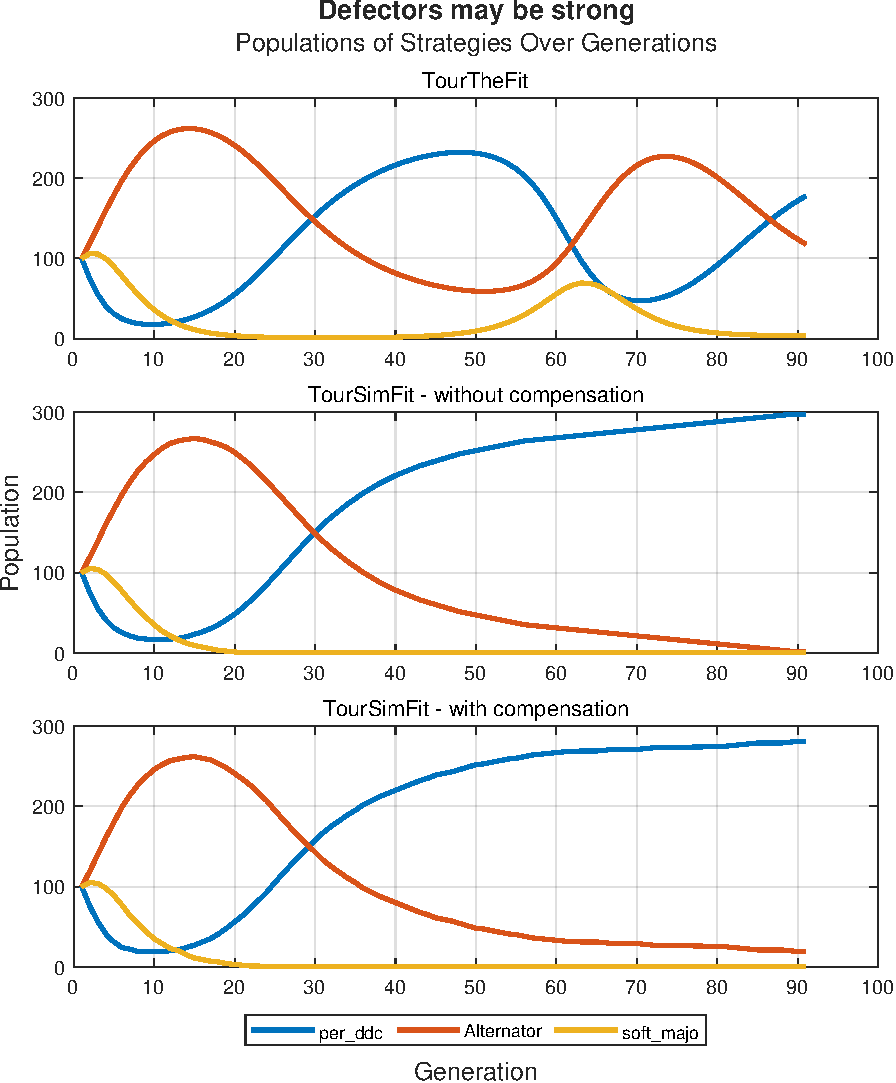
\includegraphics[scale=0.8]{Defectors may be strong.pdf}
	      \caption{Defectors may be strong}
	      \label{fig:2dmesh}
	\end{figure}
\subsubsection{2η Προσομοίωση - Μονότονη Σύγκλιση}
Στο εξής παρουσιάζονται τα αποτελέσματα για τις προσομοιώσεις που χρησιμοποιούν οι Mathieu et al ώστε να ταξινομήσουν τα γραφήματα σε 5 κατηγορίες, η πρώτη από τις οποίες είναι η μονότονη σύγκλιση των πληθυσμών. Πρόκειται για την πιο συχνή μορφή που προκύπτει, καθώς οι ταλαντώσεις που παρουσιάζονται παρακάτω είναι αρκετά ευαίσθητες ως προς τις αρχικές συνθήκες. Τα αποτελέσματα τόσο της θεωρητικής ανάλυσης όσο και των 2 προσομοιώσεων είναι πανομοιότυπα με αυτά των Mathieu et al, με μοναδική διαφορά τον ελάχιστα διαφορετικό τελικό πληθυσμό στην περίπτωση του compensation, που οφείλεται και πάλι στο τυχαίο στοιχείο. Η κατάταξη, ωστόσο, των στρατηγικών παραμένει ίδια.
	\begin{figure}[h]
	      \centering
	      \includegraphics[scale=0.8]{Monotonous Convergence.pdf}
	      \caption{Monotonous Convergence}
	      \label{fig:2dmesh}
	\end{figure}
\subsubsection{3η Προσομοίωση - Φθίνουσες Ταλαντώσεις}
Η επόμενη κατηγορία αποτελεσμάτων του paper είναι η φθίνουσες ταλαντώσεις πληθυσμών. Τα αποτελέσματα σε αυτήν την περίπτωση είναι πανομοιότυπα με αυτά των Mathieu et al και για τις τρεις περιπτώσεις που παρουσιάζονται. Οι αρχικοί πληθυσμοί στη συγκεκριμένη περίπτωση είναι αρκετά μεγάλοι, οπότε ο ένας ή δύο παίκτες που αντίθενται τυχαία στην περίπτωση του compensation δεν αλλάζουν αισθητά την πορεία της συνάρτησης.
	\begin{figure}[h]
	      \centering
	      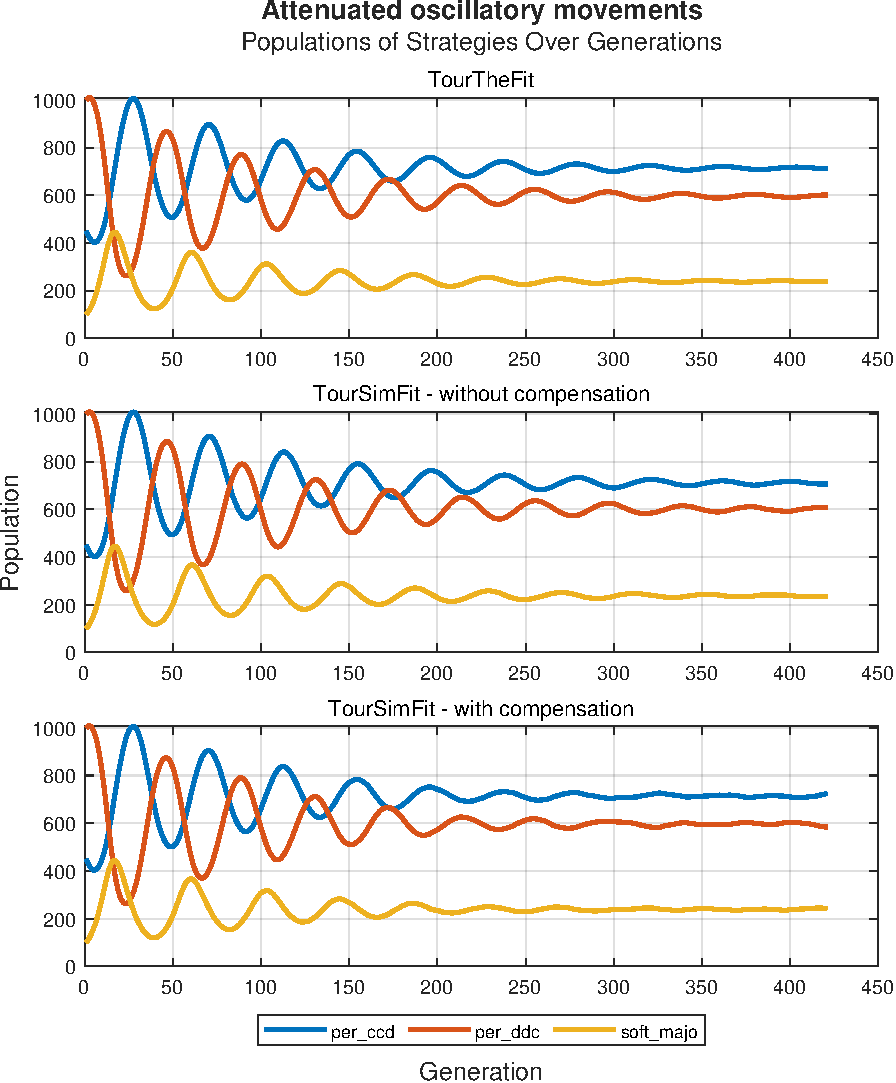
\includegraphics[scale=0.8]{Attenuated oscillatory movements.pdf}
	      \caption{Attenuated oscillatory movements}
	      \label{fig:2dmesh}
	\end{figure}
\subsubsection{4η Προσομοίωση - Περιοδικές Κινήσεις}
Τρίτη περίπτωση είναι η εμφάνιση περιοδικών κινήσεων/ταλαντώσεων, δίχως αύξηση ή μείωση των πλατών των ταλαντώσεων. Η εικόνα αυτή παρουσιάζεται σε γενικές γραμμές όταν υπάρχουν 3 στρατηγικές με τη λογική "πέτρα-ψαλίδι-χαρτί": η 1η "νικάει" τη 2η που "νικάει" την 3η που "νικάει" την 1η. Στη συγκεκριμένη περίπτωση, η per\_ccd νικάει τη soft\_majo που νικάει την per\_ddc που νικάει τη per\_ccd. Με κατάλληλους, λοιπόν, αρχικούς πληθυσμούς παρατηρούνται τα παρακάτω αποτελέσματα. Η θεωρητική ανάλυση δείχνει ότι η ταλάντωση στην πραγματικότητα σβήνει - πρόκειται για φθίνουσα ταλάντωση όπως πριν. Αυτό οφείλεται στο γεγονός ότι σε διακριτές περιπτώσεις, όπως αυτές των προσομοιώσεων, γίνεται βέβαιο με κατάλληλες επιλογές ότι θα βρεθούμε σε κατάσταση ίδια με παρελθοντική, και άρα ότι θα υπάρξει επανάληψη/ταλάντωση. Ωστόσο, στη θεωρητική ανάλυση, αυτό δε συμβαίνει ("απειρία" καταστάσεων λόγω της αριθμητικής με δεκαδικούς), και άρα παρατηρείται η απόσβεση της ταλάντωσης. Η TourSimFit χωρίς compensation αποφέρει πάλι ίδια αποτελέσματα με τους Mathieu et al, ενώ η περίπτωση με compensation, αν και αντιαισθητική στην όψη, αποτυπώνει επίσης την ταλάντωση, ακόμα και με την αισθητή ύπαρξη θορύβου λόγω της τυχαιότητας (τα πλάτη των ταλαντώσεων είναι μικρά, άρα ακόμα και η προσθήκη ενός ή δύο έξτρα παικτών έχει αισθητό αποτέλεσμα).
	\begin{figure}[h]
	      \centering
	      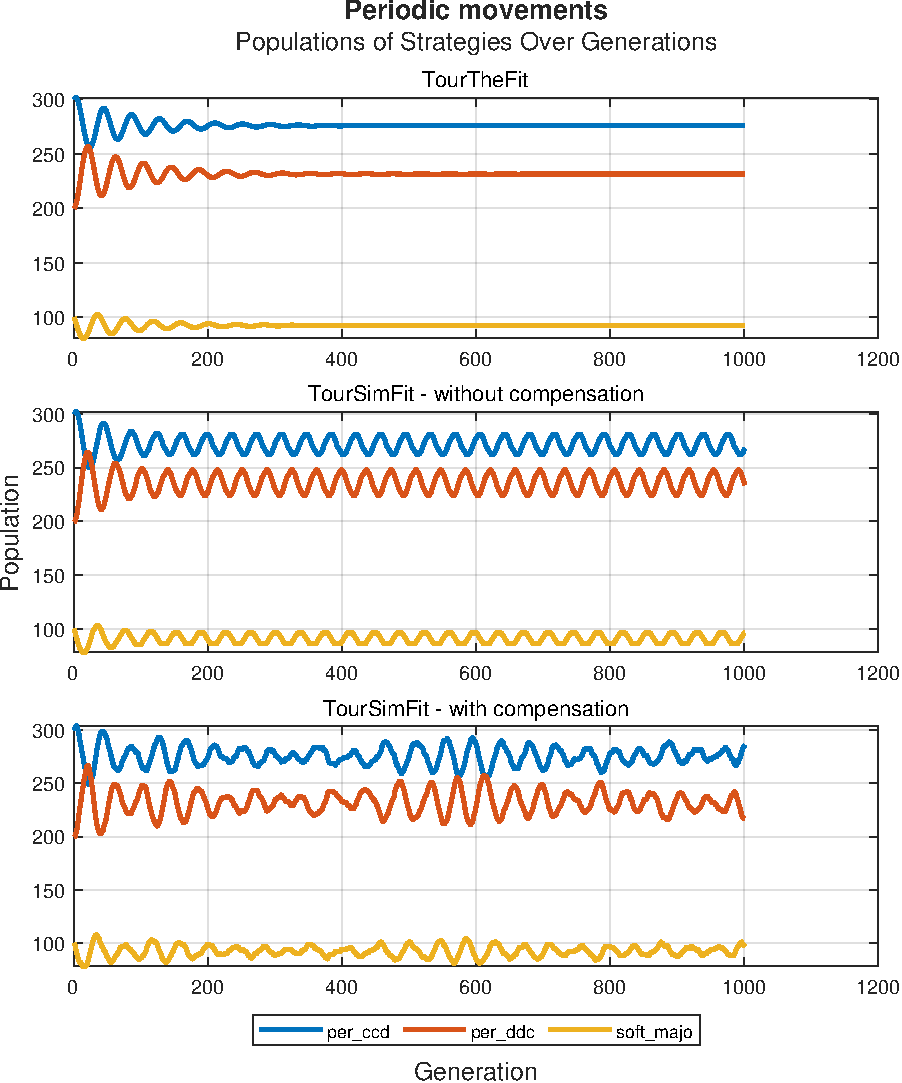
\includegraphics[scale=0.8]{Periodic movements.pdf}
	      \caption{Periodic movements}
	      \label{fig:2dmesh}
	\end{figure}
\subsubsection{5η Προσομοίωση - Αύξουσες Ταλαντώσεις}
Από τις πλέον μη αναμενόμενες περιπτώσεις είναι αυτή των αυξουσών ταλαντώσεων. Με κατάλληλη επιλογή πίνακα απολαβής, στρατηγικών και αρχικών πληθυσμών, είναι δυνατόν να παρατηρηθεί το φαινόμενο αυτό. Δοκιμάστηκε ο πληθυσμός ως έχει και τα αποτελέσματα δεν ήταν τα επιθυμητά. Έτσι, μεταβλήθηκε ο πίνακας απολαβών σε $B = \begin{bmatrix} 3 & 0 \\4.72 & 1 \end{bmatrix}$ (με δοκιμή και σφάλμα, γνωρίζοντας τη γενική κατεύθυνση στην οποία έπρεπε να κινηθεί ο πίνακας) και τελικά παρατηρήθηκε στην περίπτωση TourSimFit χωρίς compensation αποτέλεσμα πολύ όμοιο με αυτό του paper. Ωστόσο, για την ίδια τιμή του $B$ και τις περιπτώσεις της TourTheFit και TourSimFit με compensation παρατηρούνται ελαφρώς φθίνουσες ταλαντώσεις, κάτι που φανερώνει δύο αλήθειες για τις περιπτώσεις των αυξουσών ταλαντώσεων. Πρώτον, προκύπτουν από πληθυσμούς που δύνανται να εμφανίσουν κανονικές ταλαντώσεις, με κατάλληλη μεταβολή του πίνακα κερδών. Δεύτερον, είναι ιδιαίτερα ευαίσθητες περιπτώσεις που με ακόμα και ελάχιστη μετατροπή της δυναμικής (όπως π.χ. τη λογική του compensation) καταρρέουν πίσω σε κανονική ή φθίνουσα ταλάντωση. Πολύ πιθανόν για κατάλληλη επιλογή του $B$ να μετατρέπονται και οι περιπτώσεις TourTheFit και TourSimFit με compensation σε αύξουσα ταλάντωση, αλλά κρίθηκε πιο σημαντικό για την εργασία να παρουσιαστεί αυτή η απόκλιση στα αποτελέσματα.
	\begin{figure}[h]
	      \centering
	      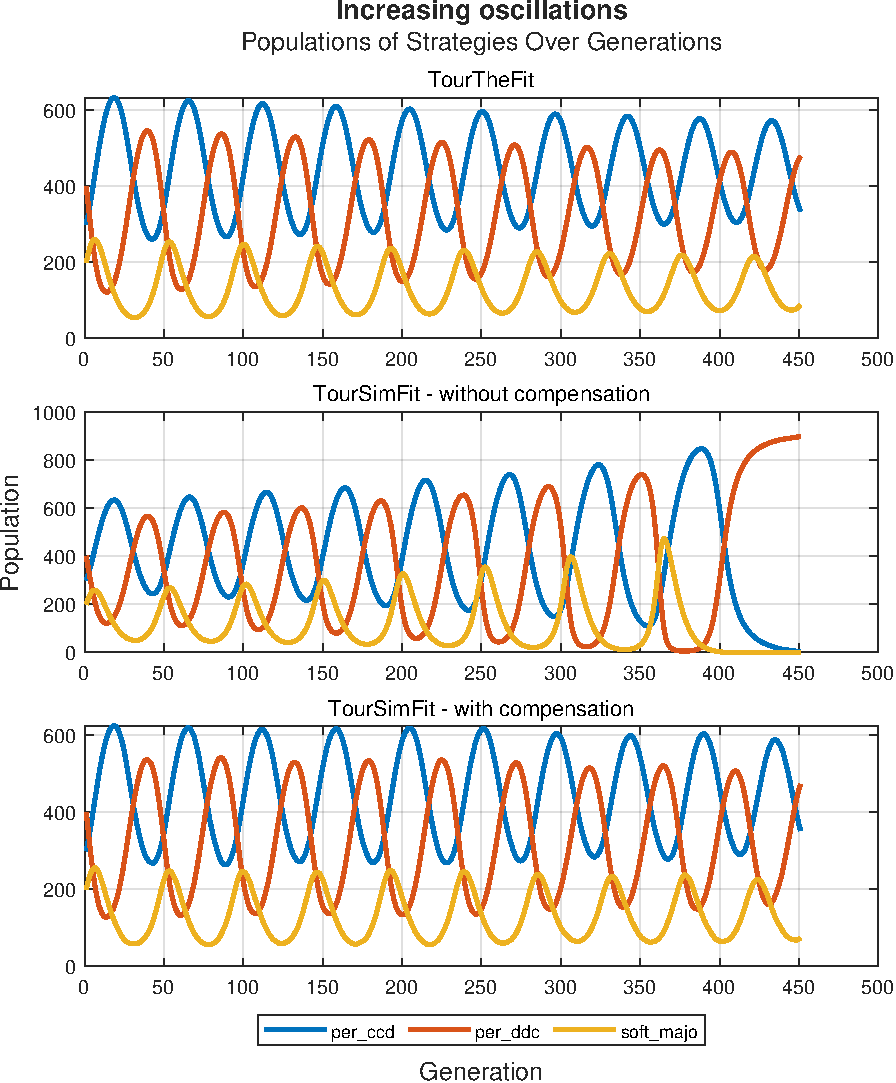
\includegraphics[scale=0.8]{Increasing oscillations.pdf}
	      \caption{Increasing oscillations}
	      \label{fig:2dmesh}
	\end{figure}
\subsubsection{6η Προσομοίωση - Χάος/Διαταραγμένες Ταλαντώσεις}
Τελευταία περίπτωση που παρουσιάζεται στο paper είναι αυτή των διαταραγμένων ταλαντώσεων. Οι συγγραφείς του paper ορθά διστάζουν να τη χαρακτηρίσουν ως πραγματικά χαοτική περίπτωση, διότι, λόγω της διακριτής φύσης της προσομοίωσης, κάθε τέτοια συμπεριφορά μετά από ικανό αριθμό γενεών είτε φτάνει σε ισορροπία είτε απλώς επαναλαμβάνεται. Τα αποτελέσματα, βέβαια, της συγκεκριμένης προσομοίωσης, μοιάζουν αρκετά χαοτικά στο μάτι. Πάλι, η περίπτωση TourSimFit δίχως compensation ανταποκρίνεται πλήρως στα αποτελέσματα του paper. Αντιθέτως, λόγω πάλι της ευαισθησίας του φαινομένου, οι περιπτώσεις της θεωρητικής ανάλυσης και της πραγματικής προσομοίωσης με compensation διαφοροποιούνται σημαντικά, διότι δεν εμφανίζουν τη χαώδη συμπεριφορά γύρω στη γενιά 140 όπως στην περίπτωση του paper. Ωστόσο, προβλέπουν την παραμονή στη ζωή των στρατηγικών per\_ccccd και Prober, αλλά και τις τιμές στις οποίες φαίνεται να τείνουν οι πληθυσμοί της περίπτωσης TourSimFit χωρίς προσομοίωση.
	\begin{figure}[h]
	      \centering
	      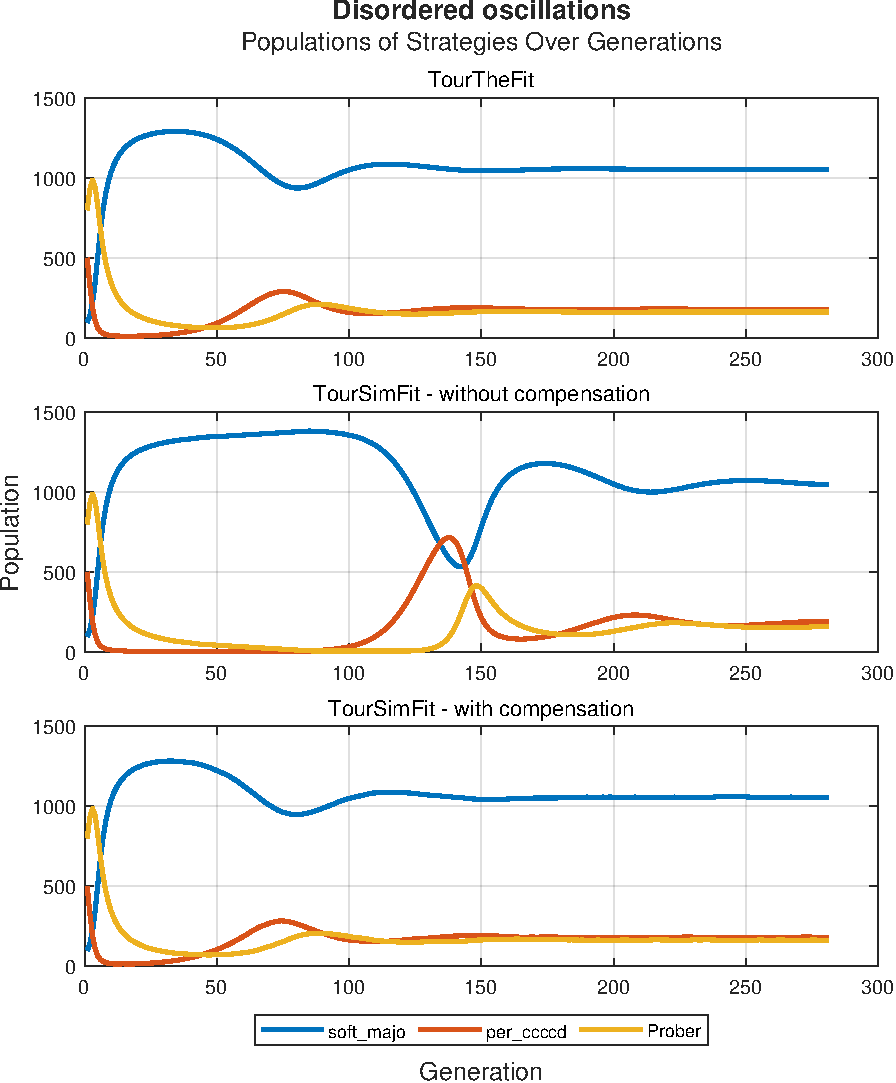
\includegraphics[scale=0.8]{Disordered oscillations.pdf}
	      \caption{Disordered oscillations}
	      \label{fig:2dmesh}
	\end{figure}

\section{Imitation Dynamics}

\subsection{Η συνάρτηση TourSimImi}

\subsubsection{1η Προσομοίωση}

\subsection{Η συνάρτηση TourTheImi}

\subsubsection{1η Προσομοίωση - Παράδειγμα χρήσης των TourTheImi και AnalyzeMarkovChain}
	\begin{figure}[H]
	      \centering
	      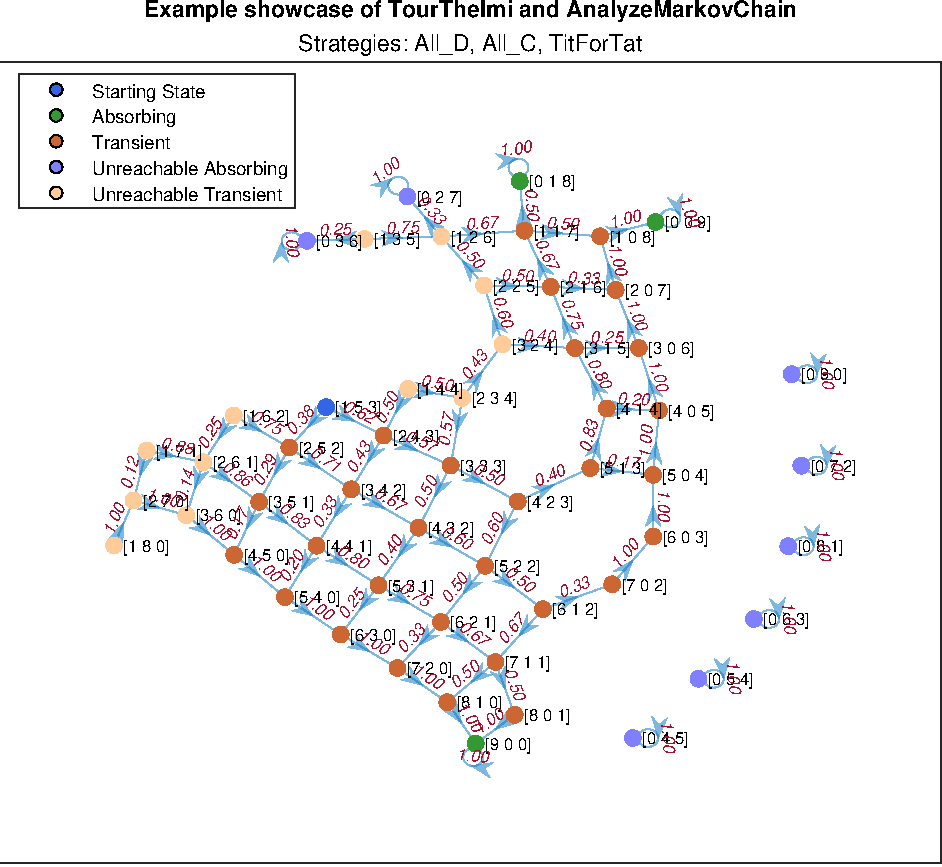
\includegraphics[width=0.95\textwidth]{Example showcase of TourTheImi and AnalyzeMarkovChain.pdf}
	      \caption{Example showcase of TourTheImi and AnalyzeMarkovChain}
	      \label{fig:2dmesh}
	\end{figure}
\subsubsection{2η Προσομοίωση - Δοκιμή προεπιλεγμένης μεθόδου (Individual) για τον προσδιορισμό της καλύτερης στρατιγίκης}
	\begin{figure}[H]
	      \centering
	      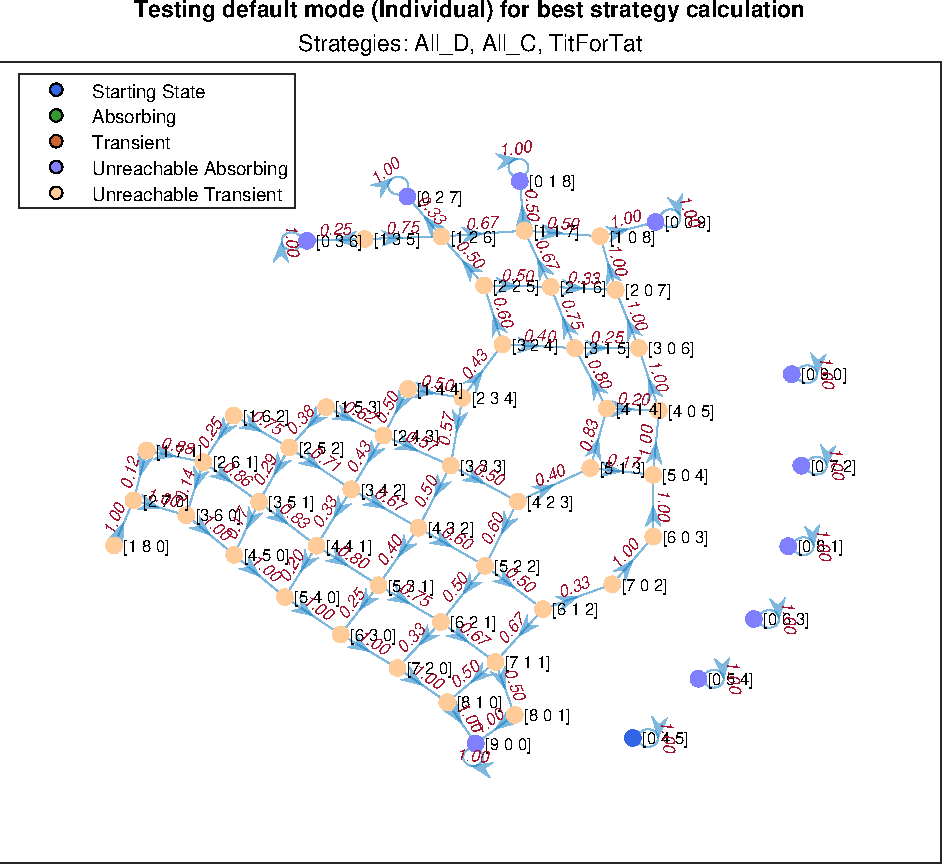
\includegraphics[width=0.95\textwidth]{Testing default mode (Individual) for best strategy calculation.pdf}
	      \caption{Testing default mode (``Individual'') for best strategy calculation.pdf}
	      \label{fig:2dmesh}
	\end{figure}
\subsubsection{3η Προσομοίωση - Δοκιμή  μεθόδου ``Total'' για τον προσδιορισμό της καλύτερης στρατιγίκης}
	\begin{figure}[H]
	      \centering
	      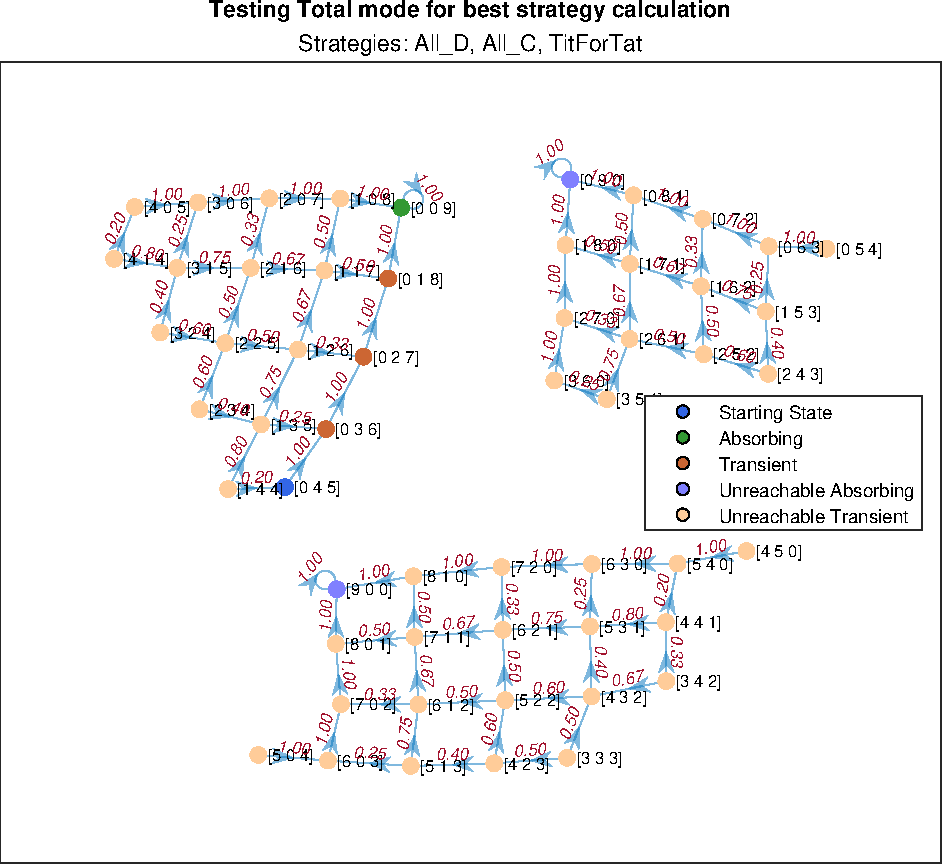
\includegraphics[width=0.95\textwidth]{Testing Total mode for best strategy calculation.pdf}
	      \caption{Testing ``Total'' mode for best strategy calculation.pdf}
	      \label{fig:2dmesh}
	\end{figure}

\section{Τελικά Συμπεράσματα}

\newpage
\listoffigures\addcontentsline{toc}{section}{Κατάλογος σχημάτων}
\end{document}